The last prototype developed for TRITIUM was TRITIUM-IFIC 2, marked as A in Figure \ref{fig:TritiumIFIC2}. This prototype, built in the IFIC workshop, consists of a cylindrical Teflon vessel, shown in Figure \ref{fig:Tritium-IFIC2_vessels}, with a similar shape to that of the TRITIUM-Aveiro prototype. The internal length and diameter of the Teflon vessel were $210~\mm$ and $36~\mm$ respectively.

\begin{figure}[h]
\centering
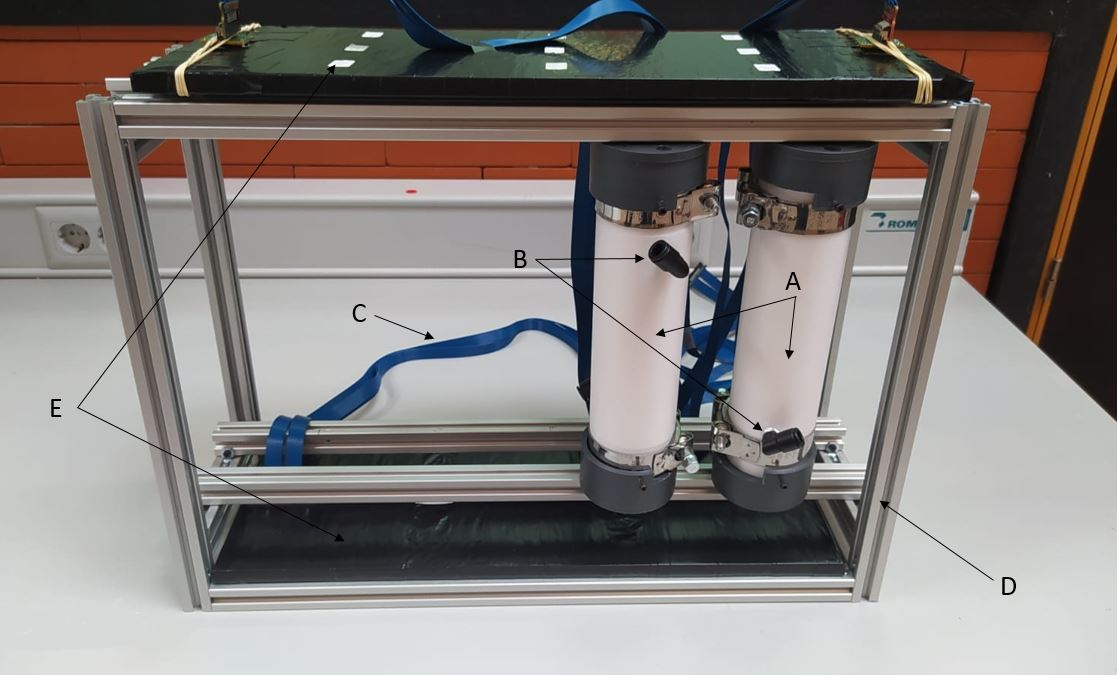
\includegraphics[scale=0.4]{5Prototypes/53FinalPrototypes/532TritiumIFIC2/Tritium_IFIC_2_full_module.jpg}
\caption{TRITIUM-IFIC 2 prototype and active veto within the metalic structure.\label{fig:TritiumIFIC2}}
\end{figure}

\begin{figure}
\centering
    \begin{subfigure}[b]{0.35\textwidth}
    \centering
    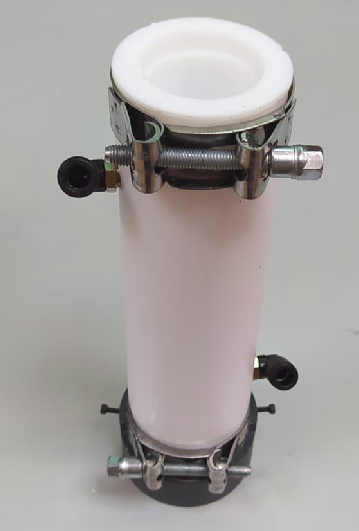
\includegraphics[width=\textwidth]{5Prototypes/53FinalPrototypes/532TritiumIFIC2/Tritium_IFIC_2_vessel1.png}  
    \caption{\label{subfig:Tritium_IFIC_2_vessel}}
    \end{subfigure}
    \hfill
    \begin{subfigure}[b]{0.3\textwidth}
    \centering
    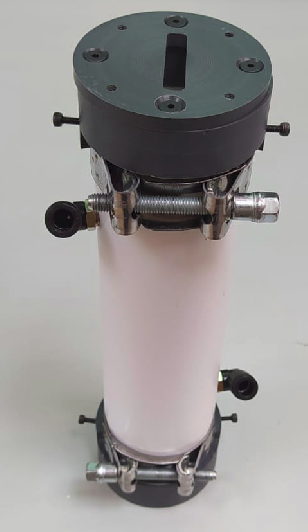
\includegraphics[width=\textwidth]{5Prototypes/53FinalPrototypes/532TritiumIFIC2/Tritium_IFIC_2_vessel2.png}  
    \caption{\label{subfig:TritiumIFIC2_vessel_with_PVC_caps}}
    \end{subfigure}
 \caption{a) TRITIUM-IFIC 2 Teflon vessel. b) TRITIUM-IFIC 2 Teflon vessel with PVC caps}
 \label{fig:Tritium-IFIC2_vessels}
\end{figure}

This prototype contains $800$ uncladded BCF-12 scintillating fiber of $200~\mm$ length. This number is larger than that of the TRITIUM-Aveiro prototype and is contained in a smaller volume. The fibers used were cleaved, polished and cleaned with the conditioning process described in section \ref{sec:CharacterizationScintillatingFibers}.

This number of fibers, which were freely arranged, just allowed water to flow through them. Two PMMA windows, located at the ends of the fiber bundle, allowed to read the scintillation light as in the TRITIUM-Aveiro prototype. 

$5~\mm$ width PMMA optical windows is sufficient to guarantee tightness since the detector works at very low water pressure. Two clamps keep the tightness of the prototype, similar to the TRITIUM-Aveiro prototype. PMMA was chosen for its optical properties, especially its transmission coefficient, which was measured for visible spectrum in the ICMOL laboratories, shown in Figure \ref{fig:PMMATransmissionSpectrum}. This transmission coefficient is approximately $95\%$ for the working wavelength ($435~\nm$). Slightly better transmission coefficients can be achieved with other materials such as quartz or sapphire but they are much more expensive.

\begin{figure}[h]
\centering
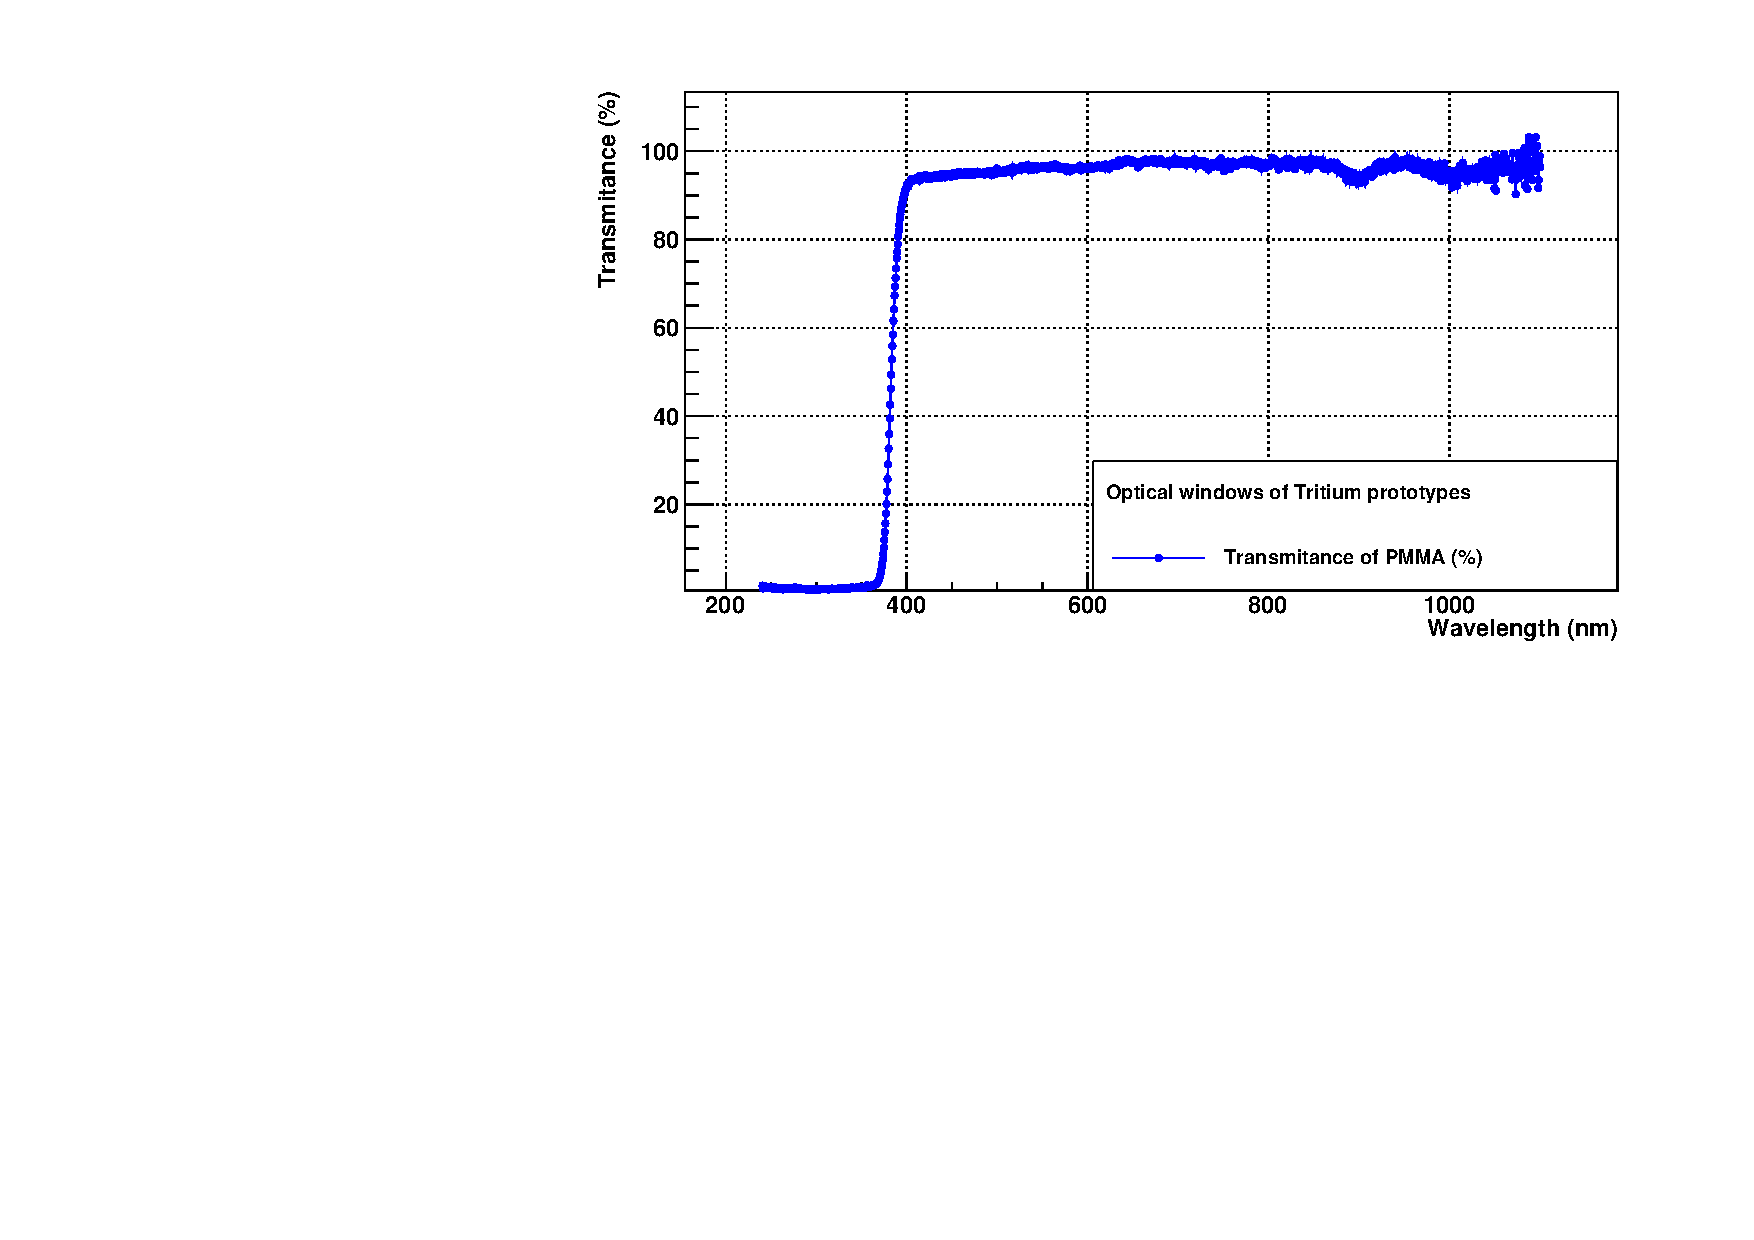
\includegraphics[scale=0.6]{5Prototypes/53FinalPrototypes/532TritiumIFIC2/TransmissionSpectrumPMMA_cut_at_low_energy.pdf}
\caption{Transmission spectrum of light by a $5~\mm$ thick of PMMA plate. (measured in the ICMOL laboratory). \label{fig:PMMATransmissionSpectrum}}
\end{figure}	

A water inlet/outlet was implemented in the Teflon vessel, shown in Figure Figure \ref{fig:Tritium-IFIC2_vessels}, to allow a constant water flux, similar to the TRITIUM-Aveiro prototype.

For the first laboratory measurements, two R8520-460 PMTs from the Hamamatsu Photonics \cite{DataSheetPMTs}, were used to compare the results to those of the previous prototypes. However, measurements of the TRITIUM-IFIC 2 prototype with SiPM arrays and PETSYS electronics have already started since the final version will use them.

%The PETSYS system is employed to read out the SiPMs used in the TRITIUM-IFIC 2 prototype to be installed in Arrocampo dam. Therefore, it is not necessary to develop a electronics chain to process and analyze the PMT signals of this prototype.

PETSYS has a graphical user interface, shown in Figure \ref{fig:GUI_PETSYS}. However, they also allow remote controll of all the different options such as supply voltage for the SiPM arrays, thresholds, etc., via computer terminal. 

\begin{figure}[h]
\centering
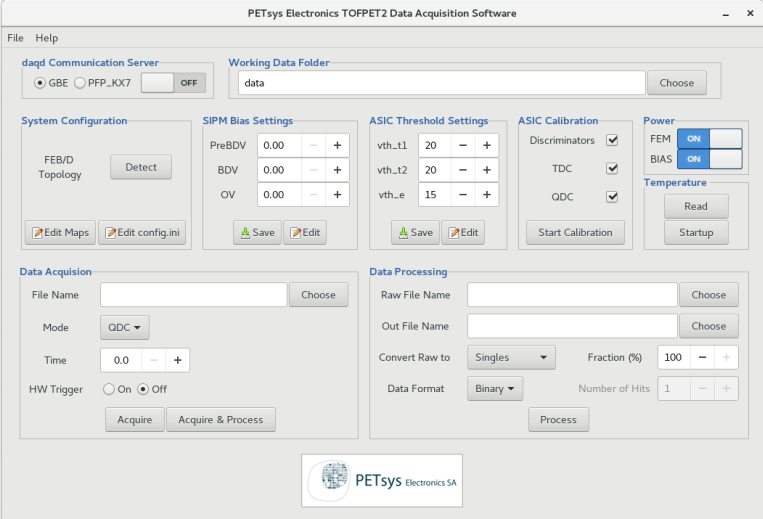
\includegraphics[scale=0.4]{5Prototypes/53FinalPrototypes/532TritiumIFIC2/GUI_PETSYS.png}
\caption{Graphical User Interface (GUI) of PETSYS.\label{fig:GUI_PETSYS}}
\end{figure}

Two PVC caps, located at both ends of the prototype were used to provide to the SiPMs a light-tight environment. An aluminum structure was designed and built to house up to 10 TRITIUM-IFIC 2 modules and two cosmic vetos, marked as D in Figure \ref{fig:TritiumIFIC2}.

The available space within the lead shielding can accommodate up to 5 structures, which means that the final TRITIUM moitor may accommodate up to 50 TRITIUM-IFIC 2 modules and 5 different cosmic vetos. As the sensitivity of the TRITIUM monitor scales with the number of TRITIUM modules used, the results obtained with the TRITIUM monitor should improve those results by a factor of $\sqrt{N}$, where N is the number of modules used.

Two identical TRITIUM-IFIC 2 prototypes were built, similar to the TRITIUM-IFIC 0 prototype. One of them was filled with ultrapure water and used to measure the background and the other was filled with a radioactive liquid source of tritium and used to measure the signal. The water volume in both cases was $82~\milli\liter$ (uncertainty of $0.05\%$).The activity of the tritium source used for this prototype was $10~\kilo\becquerel/\liter$ (uncertainty of $2.24\%$), which was prepared by diluting a sample of tritiated water in ultrapure water.

The results provided by this prototype are shown in chapter\ref{chap:ResultsPrototypes}.